\chapter{Snow Density Estimation From Full Polarimetric SAR Data}
\section{Introduction}
\label{S:1}
%The Earth's land surface is covered by more than thirty percent of seasonal snow~\citep{robinson1993global}. Snow is a medium of considerable interest to hydrology, climatology and avalanche research which has lead to the characterization of snowpack properties at various frequencies. In general, snow is electromagnetically a three component dielectric mixture of ice, water and air. Dry snow is an inhomogeneous medium consisting of ice particles and air voids, whereas wet snow consists of ice spheres embedded in an air-water medium. Snow density is an important parameter of the snowpack which influences the thermal, mechanical and optical properties of snow layers. It is thus a vital parameter for avalanche prediction~\citep{hirashima2009adjustment,brun1989investigation} and snow hydrology~\citep{rango1995revisiting,jonas2009estimating,sturm2010estimating}. 

The snow density is a complex parameter that can vary spatially, temporally and vertically within the snow pack profile~\citep{bormann2013spatial}. Wind erosion, melt-refreeze events, compaction and snow metamorphisms acting in response to internal temperature and moisture gradients~\citep{sommerfeld1970classification,colbeck1982overview} are responsible for seasonal snowpack densification. The snow particles gets reshaped into sphere like structures due to wind erosion. These sphere shaped particles then closely pack together thereby increasing the density. The melt-freeze processes~\citep{colbeck1982overview} due to temperature fluctuations is majorly responsible for snow densification. The liquid water content present in the snowpack~\citep{brun1989energy,marshall1999snow} along with the destructive snow metamorphisms occurring when vertical temperature gradients are weak~\citep{colbeck1982overview} results in smaller and rounded particles. 

As given in NS 3491-3 and EN 1991-1-3 (European Committee for Standardization, 2003) the mean density of snow is given in~Table~I~\citep{MET40}. 

\begin{table}[!h]
	\caption{Bulk weight density of snow according to EN 1991-1-3
		and NS 3491-3 (settled snow is measured several hours or days
		after its fall; old snow several weeks or months after its fall)~\citep{MET40}}
	\centering
	\begin{tabu} to 1\textwidth { X[l] X[r]}
		\toprule
		Type of snow & Bulk weight density (kg m $^{-3}$) \\ 
		\bottomrule
	\end{tabu}
	\begin{tabu} to 1\textwidth { X[l] X[r]}
		Fresh & 100 \\ 
		Settled & 200\\ 
		Old & 250-350\\
		Wet & 400 \\
		\bottomrule
	\end{tabu}
	\label{table:area_A}
\end{table}

Several works have been done with the microwave interaction of snow at various frequencies~\citep{stiles1980active,ulaby1980active,ulaby1984snowcover,rott1987possibilities,rott1988study}. The radar backscattering coefficient is a function of various parameters classified as surface parameters and radar observation parameters. The radar observation parameters include the transmission wave frequency, polarization, and incidence angle. Surface parameters include roughness, geometrical shape and dielectric properties of the target. SAR data showed its potential for snow cover monitoring in the boreal forest zone~\citep{koskinen1997use}. Several theoretical models have been developed and experimental data sets have been analyzed to relate backscattered coefficient of snow covered terrain with its physical properties~\citep{Shi95,Shi2000,shi2000depth,besic2012dry,besic2015stochastic}. All these studies have indicated that the factors which have been found to have the most profound influence on the backscatter coefficient are snow water equivalent, liquid water content and moisture content of soil. The snow surface roughness and size distribution of ice crystals are also some of the important factors and the extent of their importance is further dependent on the wavelength used and the angle of incidence. Satellite remote sensing is a key tool in monitoring the snow pack parameters over a large area. Microwave remote sensing measurements can be efficiently used to infer bulk properties of snowpack. In comparison to conventional single-channel Synthetic Aperture Radar (SAR), the introduction of SAR polarimetry can significantly improve the quality of the results. These improvements are due to the quantitative ability of polarimetric SAR to scattering mechanisms. Hence, remote sensing using polarimetric SAR data has great potential in determining the extent and the properties of snow. There are many snow and glacier studies done over the Indian Himalayan region using fully polarimetric SAR data~\citep{singh2011a,singh2012a,singh2012b,singh2014a,singh2014b}.

Many algorithms have been developed for SAR data to estimate the snow dielectric constant~\citep{Shi93,Shi95,Singh2007_spie,niang2007new,singh2010snow,surendar2013improved,bhattacharya2014snow}. The real part of the relative dielectric constant~($\varepsilon{'}$) is solely dependent on the density. Dry snow density estimates have been obtained by~\citep{Shi2000} using full-polarimetric SIR-C/XSAR L-band SAR data. This model can be applied over a large range of incident angles (10$^\circ$ - 70$^\circ$). The estimated snow density compared to field measurements shows an RMSE of 0.042 gcm$^{-3}$ and a relative error of 13$\%$. Even though they used full polarimetry data, they did not utilize the complete full-polarimetric information. However, they have only considered a first order backscattering coefficients to invert snow density. 

In this chapter a novel inversion model for snow density estimation from full-polarimetric SAR data based on G4U scattering power decomposition is proposed which utilizes the complete polarimetric information. Unlike the L-band data, the estimation of the snow density using C-band relies mainly on the scattering from the snowpack volume. Therefore the generalized volume parameter is adopted in this study. This parameter is then directly used to estimate the snowpack dielectric constant. The effective snow dielectric constant is derived using the normalized volume scattering power which is then used in a semi-empirical equation to estimate the snow density. The results obtained from the proposed method are validated with in-situ measurements which were obtained in near-real time along with the satellite pass.

\section{Methodology}
\label{S:2}
Followed by the previous section of snow wetness estimation from full polarimetry SAR data, here also the general four-component scattering power decomposition method (G4U)~\citep{singh13} is adopted to develop a new snow density estimation method. The G4U decomposition which is used in this study has the added advantage of full utilization of the polarimetric coherency phase information provided by a full-polarimetric SAR data. 

%Unlike the Freeman-Durden decomposition (FDD)~\citep{freeman98}, the Yamaguchi 4-component decomposition (Y4O)~\citep{Yamaguchi05} and the Yamaguchi 4-component decomposition with rotation (Y4R)~\citep{YAMAGUCHI2011}, which only uses 55.5$\%$, 66.6$\%$ and 75$\%$ of the polarimetric phase information respectively whereas the G4U utilizes 100$\%$ of the polarimetric phase information which is implemented by a double unitary transformation of the coherency matrix~(\ref{eq:g4u_decomposition_1} and~\ref{eq:g4u_decomposition_2}), 
%
%\begin{subequations}
%\begin{multline}
% \left\langle\mathbf{[T(\theta)]}\right\rangle = \left[U(\theta)\right]\Bigl(f_{s}\left\langle\mathbf{[T]}\right\rangle_{surface} +  f_{d}\left\langle\mathbf{[T]}\right\rangle_{double} + f_v\left\langle\mathbf{[T]}\right\rangle_{vol} \\ + f_{c}\left\langle\mathbf{[T]}\right\rangle_{helix}\Bigr)\left[U(\theta)\right]^{\dagger}
%\label{eq:g4u_decomposition_1}
%\end{multline}
%\begin{equation}
%\left\langle\mathbf{[T(\phi)]}\right\rangle = \left[U(\phi)\right]\left\langle\mathbf{[T(\theta)]}\right\rangle\left[U(\phi)\right]^{\dagger} = \left[ \begin{array}{ccc}
%T_{11} & T_{12} & T_{13} \\
%T_{21} & T_{22} & 0 \\
%T_{31} & 0 & T_{33}
%\end{array}\right] 
%\label{eq:g4u_decomposition_2}
%\end{equation}
%\begin{equation}
%\left[U(\theta)\right] = \left[ \begin{array}{ccc}
%1 & 0 & 0 \\
%0 & \mbox{cos}2\theta & \mbox{sin}2\theta \\
%0 & -\mbox{sin}2\theta & \mbox{cos}2\theta
%\end{array}\right];  \quad
%\left[U(\phi)\right] = \left[ \begin{array}{ccc}
%1 & 0 & 0 \\
%0 & \mbox{cos}2\phi & j\mbox{sin}2\phi \\
%0 & j\mbox{sin}2\phi & \mbox{cos}2\phi
%\end{array}\right]
%\label{eq:utheta_and_uphi}
%\end{equation}
%\end{subequations}
%where $\dagger$ denotes complex conjugation and transposition, $\left[U(\theta)\right]$ and $\left[U(\phi)\right]$ denotes the real and the complex unitary transformation matrices respectively~(\ref{eq:utheta_and_uphi}) and $\left\langle\mathbf{[T(\theta)]}\right\rangle = \left[U(\theta)\right]\left\langle\mathbf{[T]}\right\rangle\left[U(\theta)\right]^{\dagger}$ denotes the measured coherency matrix after real orientation compensation. The $f_{s}$, $f_d$, $f_v$ and $f_{c}$ are the corresponding scattering coefficients of the expansion matrices, $\left\langle\mathbf{[T]}\right\rangle_{surface}$, $\left\langle\mathbf{[T]}\right\rangle_{double}$, $\left\langle\mathbf{[T]}\right\rangle_{vol}$ and $\left\langle\mathbf{[T]}\right\rangle_{helix}$ respectively. These coefficient are then used to estimate the surface ($P_s$), double-bounce ($P_d$), volume ($P_v$) and the helix ($P_c$) scattering powers. 
In this work the scattering by snow particles is modeled in terms of their polarizability.The volume scattering matrix defined for a single particle is defined as,
\begin{equation}
	[S_{vol}]=\left[\begin{array}{cc}
		S_{HH}^{vol} & 0 \\
		0 & S_{VV}^{vol}
	\end{array}\right] = S_{HH}^{vol}\left[\begin{array}{cc}
	1 & 0 \\
	0 & A_{p}
\end{array}\right]
\label{eq:scattering_matrix_fung_sd}
\end{equation}
where $A_{p}$ is known as the particle anisotropy.The anisotropy can also be interpreted in terms of the particle geometry and can be defined as the ratio of the principal values of polarizability~\cite{cloude2009polarisation}. In general, the anisotropy parameter can be used to a certain degree of reliability as a reference for the particle shape. However, the anisotropy parameter is also bounded by the dielectric constant ($\varepsilon$) of the particle and is bounded by,
\begin{equation}
	\frac{1}{\varepsilon{'}_{v}}<A_{p}<\frac{\varepsilon{'}_{v} + 1}{2}.
	\label{eq:anisotropy_sd}
\end{equation}
In order to have a volume scattering from a random cloud of snow particles, the volume scattering matrix defined in~(\ref{eq:scattering_matrix_fung_sd}) should be arbitrarily rotated about the line of sight by an angle $\theta$ as,
\begin{equation}
	[S_{vol}]=S_{HH}^{vol}\left[\begin{array}{cc}
		\mbox{cos}(\theta) & \mbox{sin}(\theta) \\
		-\mbox{sin}(\theta) & \mbox{cos}(\theta)
	\end{array}\right]\left[\begin{array}{cc}
	1 & 0 \\
	0 & A_{p}
\end{array}\right]\left[\begin{array}{cc}
\mbox{cos}(\theta) & -\mbox{sin}(\theta) \\
\mbox{sin}(\theta) & \mbox{cos}(\theta)
\end{array}\right].
\label{eq:rotated_volume_scattering_matrix_sd}
\end{equation}
for which the volume coherency matrix $[T(\theta)]_{vol}$ can be written as,
\begin{equation}
	[T(\theta)]_{vol}=\frac{1}{2}\left|S_{HH}^{vol}\right|^2\left[\begin{array}{ccc}
		|1+A_{p}|^2 & (1 + A_{p})\mbox{cos}2\theta & -(1 + A_{p})\mbox{sin}2\theta    \\
		(1 + A_{p})^*\mbox{cos}2\theta & |1-A_{p}|^2\mbox{cos}^22\theta  & -|1-A_{p}|^2\frac{\mbox{sin}4\theta}{2}   \\ 
		-(1 + A_{p})^*\mbox{sin}2\theta & -|1-A_{p}|^2\frac{\mbox{sin}4\theta}{2} & |1-A_{p}|^2\mbox{sin}^22\theta
	\end{array}\right].
	\label{eq:coh_matrix_sp_sd}
\end{equation}
The volume scattering coherency matrix in~(\ref{eq:coh_matrix_sp_sd}) is averaged over all possible angles $\theta$ to obtain the volume scattering coherency matrix of a random cloud of small spheroid particles in one resolution cell as,
\begin{equation}
	\left\langle[T]\right\rangle_{vol}^{snow}=\int[T(\theta)]_{vol}p(\theta)d\theta
	\label{eq:average_coherency_matrix_sd}
\end{equation}
for uniformly distributed snow particles, 
\begin{equation}
	p(\theta)=\frac{1}{2\pi} \quad; 0<\theta<2\pi
	\label{eq:uniform_distrbn_sd}
\end{equation}
The average snow volume coherency matrix~(\ref{eq:volume_coherency_matrix_sd}) can be written in terms of generalized volume parameter ($|\gamma|^2$), 
\begin{equation}
	\left\langle\mathbf{[T]}\right\rangle_{vol}^{snow} = f_{v}\left[ \begin{array}{ccc}
		|\gamma|^{2} & 0 & 0 \\
		0 & \frac{1}{2} & 0 \\
		0 & 0 & \frac{1}{2}
	\end{array}\right].
	\label{eq:volume_coherency_matrix_sd}
\end{equation}
with the volume scattering coefficient as,
\begin{equation}
	f_{v} = \frac{1}{2}|\gamma_{HH}-\gamma_{VV}|^{2}f(\theta_{i},\theta_{r},\omega,\tau,P)
	\label{eq:fv_sw}
\end{equation}
where $\theta_{i}$ and $\theta_{r}$ are the local incidence and refractive angles, $\omega=\kappa_{s}/\kappa_{e}$ is the snow volume albedo, defined as the ratio of the scattering $\kappa_{s}$ and the extinction coefficient $\kappa_{e}$, $\tau$ is the optical depth ($\tau=\kappa_{e}d$) where $d$ is the snow depth, $P$ is the Rayleigh scattering phase function and,
\begin{equation}
	|\gamma|^2 = \frac{|\gamma_{HH} + \gamma_{VV}|^2}{|\gamma_{HH} - \gamma_{VV}|^2} = \frac{|1 + A_{p}|^2}{|1 - A_{p}|^2}.
	\label{eq:gammasquare_sd}
\end{equation}
where $\gamma_{HH}$ and $\gamma_{VV}$ are the Fresnel transmission coefficients for HH and VV polarizations respectively,
\begin{subequations}
	\begin{align}
		\gamma_{HH} =& \frac{2\sqrt{\varepsilon{'}_{v} - \mbox{sin}^2\theta_{i}}}{\mbox{cos}\theta_{i} + \sqrt{\varepsilon{'}_{v} - \mbox{sin}^2\theta_{i}}} \\
		\gamma_{VV} =& \frac{2\sqrt{\varepsilon{'}_{v} - \mbox{sin}^2\theta_{i}}}{\varepsilon{'}_{v}\mbox{cos}\theta_{i} + \sqrt{\varepsilon{'}_{v} - \mbox{sin}^2\theta_{i}}}
	\end{align}
	\label{eq:fresnel_trans_coefficients_sd}
\end{subequations}
the local incidence angle $\theta_{i}$ should be converted into the local refractive angle $\theta_{r}$ using the Snell's law.
%Since $A_{p}$ is bounded, therefore $|\gamma|^2$ is also bounded as,
%\begin{equation}
%\left|\frac{\varepsilon_{v}+1}{\varepsilon_{v}-1}\right|^2 < |\gamma|^2 < \left|\frac{\varepsilon_{v}+3}{\varepsilon_{v}-1}\right|^2
%\end{equation}
By assuming that the double-bounce scattering is negligible in wet snow, the generalized volume parameter $|\gamma|^2$ is derived~\cite{singh2013b} as,
\begin{equation}
	|\gamma|^2 = \frac{T_{11}(\theta)}{2T_{33}(\theta)-f_c} - \frac{|T_{12}(\theta)+T_{13}(\theta)|^{2}}{(2T_{33}(\theta)-f_{c})(T_{22}(\theta)-T_{33}(\theta)}
	\label{eq:gamma_square_coherency_elememts_sd}
\end{equation}
where $f_{c}$ is the helix scattering coefficient given as,
\begin{equation}
	f_{c}=2|\mbox{Im}\{T_{23}(\theta)\}|.
	\label{eq:helix_scattering_coefficient_sd}
\end{equation}
The snow volume dielectric constant is then estimated by equating~(\ref{eq:gammasquare_sd}) and~(\ref{eq:gamma_square_coherency_elememts_sd}).
 
The estimated snowpack volume dielectric constant is normalized with the volume scattering power fraction ($\omega=P_v/TP$) estimated from the G4U decomposition. This normalized (effective) snowpack dielectric constant ($\varepsilon_{e}{'}=\omega.\varepsilon_{v}{'}$) is then used in the Looyenga's semi-empirical dielectric equation~\citep{looyenga1965dielectric} to estimate the snow density ($\rho_s$). The flowchart of the proposed methodology is shown in Fig.~\ref{fig:methodology}. 

\begin{equation}
\varepsilon_{e}{'}=1.0 + 1.5995\rho_s + 1.861\rho_s^{3}
\label{eq:looyenga}
\end{equation}

\begin{figure*}[!th]
	\centering
	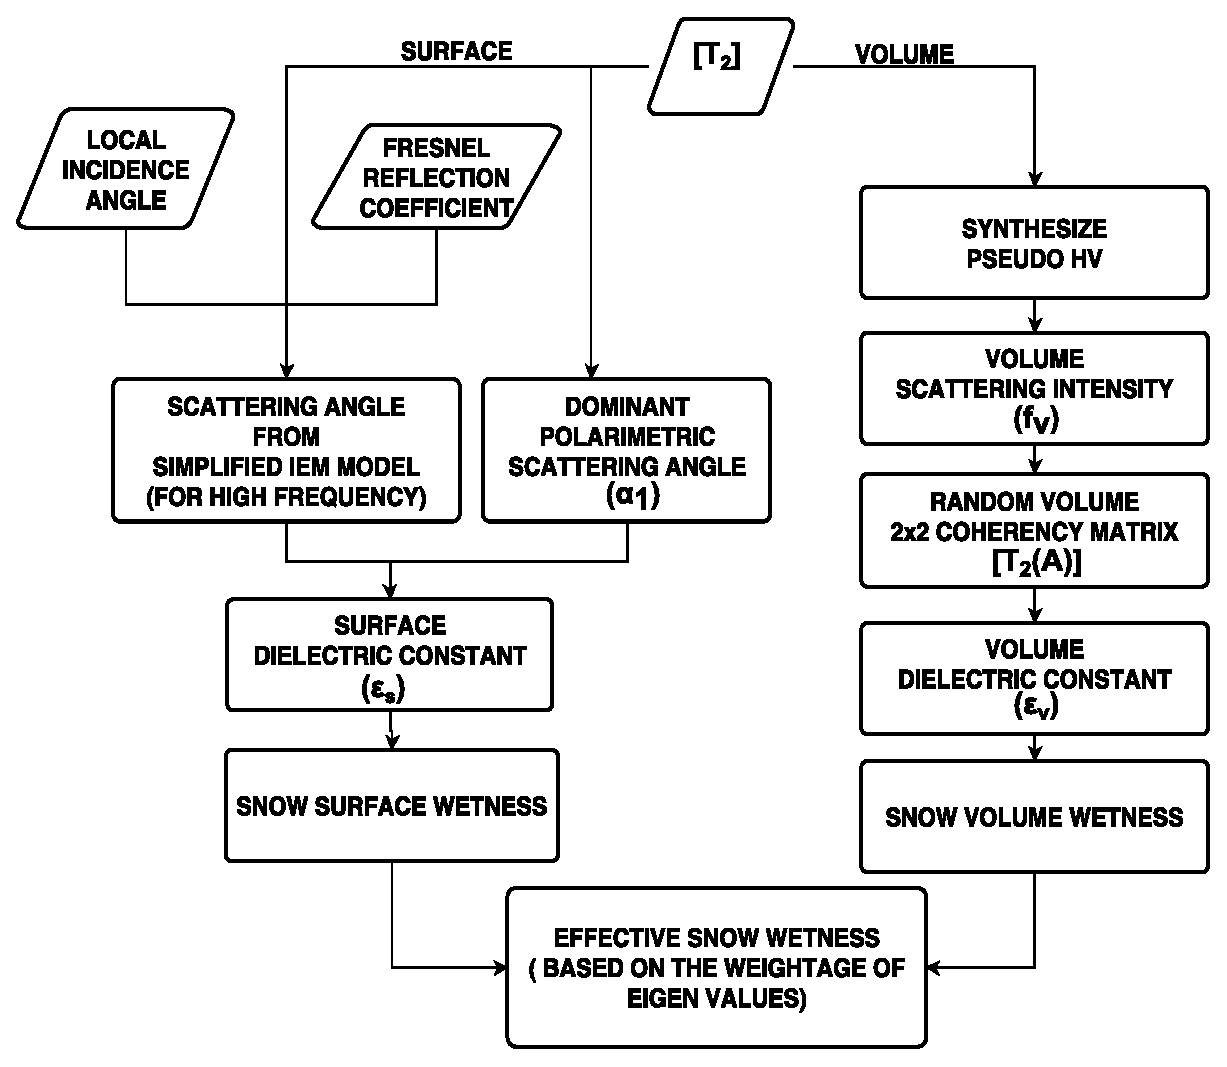
\includegraphics[width=0.6\textwidth]{Figures_sd/flow_chart}
	\caption{Flowchart of the proposed methodology}
	\label{fig:methodology}
\end{figure*}

In this proposed method, the generalized volume parameter utilizes the full-polarimetric SAR measurements from the snowpack. Hence, this parameter is able to take care of various snow conditions. On the other hand, the scattering powers from the snowpack volume is a function of the penetration depth, the grain size, the snow wetness etc. So, the generalized volume parameter combined with the scattering power is able to correctly quantify the snowpack density. During February in the Indian Himalayan region more than 90 $\%$ of the study area was completely covered with snow and our method was directly applied to the area. There was no masking was used in this study to classify a area into wet/dry snow/snow free areas. The classification of wet or dry snow was not required because the proposed model takes into account different scattering mechanism contribution associated with different snow conditions while calculating the effective density. 
\section{Study area and dataset}
\label{S:3}
The study area comprised of snow cover over an undulating rough terrain with sparse vegetation. This area is a part of the Beas and the Chandra Bhaga catchment which lies in the Kullu district of Himachal Pradesh, India. It is geographically located between the latitudes of 32$^\circ$ 15' N and 32$^\circ$ 30' N, and between the longitudes of 77$^\circ$ E and 77$^\circ$ 15' E. The Snow and Avalanche Study Establishment (SASE) under Ministry of Defense, Government of India, maintains three manual observatories at Solang, Dhundhi and Bahang which are located at an altitude of 2006~m, 2446~m and 2896~m respectively. In fact, the altitude of the entire study area varies from 2000~m to 5000~m. According to the Forest Survey of India (FSI) report in 2011~\citep{FSI2011}, less than 17$\%$ of the entire state of Himachal Pradesh (55,673~km$^2$) is covered with dense forest. The study area considered for this work is only 126~km$^2$ over the state of Himachal Pradesh, India. In the Indian Himalayan region the snowfall generally occurs during December to March from an altitude of 2000 m above the mean sea level. The mean minimum temperature in the month of January is around -15$^\circ$C-0$^\circ$C and the mean maximum temperature in the month of June is around 20$^\circ$C-30$^\circ$C. The mean high and low temperatures in the month of February over the study area is around 11.7$^\circ$C  and -0.7$^\circ$C respectively.

\begin{figure*}[!th]
	\centering
	\subfloat[]{\includegraphics[width=\columnwidth]{Figures_sd/sa_final}} \\
	\subfloat[]{\includegraphics[width=0.7\columnwidth]{Figures_sd/Study}}
	\caption{(a) Study area with location of the three observatories shown in the optical Google earth image. Courtesy: Google earth; (b) The zoning map of the study area. }
	\label{fig:study_area}
\end{figure*}

\begin{table}[!th]
	\caption{Data Acquisition Table}
	\begin{center}
		\begin{tabular}{|c|c|p{3cm}|c|p{2cm}|} \hline
			No. & Date & Acquisition Time (UTC+5:30h) & Pass & Incidence Angle ($^\circ$) \\ \hline \hline
			1 &  7 Feb. 2012 & 6:18 AM & Descending & 41.9--43.3\\ \hline
			2 &  8 Feb. 2013 & 6:14 AM & Descending & 46.0--47.2\\ \hline
			3 & 18 Feb. 2014 & 6:29 PM & Ascending & 44.4--45.7\\ \hline \hline
			4 & 29 Jan. 2015 & 6:14 AM & Descending & 46.0--47.2 \\ \hline
			5 & 22 Feb. 2015 & 6:14 AM & Descending & 46.0--47.2 \\ \hline
			6 & 18 Mar. 2015 & 6:14 AM & Descending & 46.0--47.2 \\ \hline
		\end{tabular}
	\end{center}
	\label{table:data acquisition_sd}
\end{table}

Field campaigns were conducted to collect near-real time in-situ measurements with the Radarsat-2 fine resolution quad polarimetric (FQ) data acquisitions for consecutive three winter seasons from 2012 to 2014 is shown in Table~\ref{table:data acquisition_sd}. The study area is outlined in blue and the three observatories where the field campaigns were conducted are marked (green star) in Fig.~\ref{fig:study_area}. The 3x3 coherency matrix was generated from the single-look complex Radarsat-2 full-polarimetric SAR data. A multi looking factor of 3 in the range direction and 4 in the azimuth direction were used to make the square pixel and the Lee-Refined filter is applied to remove the speckle noise. The local incidence angle map is generated while performing the Range–Doppler terrain correction using the ASTER GDEM and the Layover/Shadow areas were also masked before applying the methodology. The range and azimuthal pixel spacing were approximately 20~m (19.7~m x 20.9~m) respectively after these preprocessing.

The snow fork instrument has been used to measure the snow wetness in the field. The snow fork is a portable instrument which measures the resonant frequency, attenuation and the 3-db bandwidth~\citep{sihvola1986snow}. These measurements are then used to calculate the complex dielectric constant of snow. The snow density and the wetness are calculated using semi-empirical equations. The measurements from this instrument are reliable as it does not compress the snowpack and the measurements are easily repeatable and the results can be checked by calibration measurement in the air. These measurement were taken over the observatory areas which were almost flat. The density measurement values over the single pixel area were close enough. So in this regard an averaged value for the measurements were used to validate the snow density estimated from the SAR data.   

%\section{Results and discussion}
%\label{S:4}
%The snow density estimated by the proposed method for 7 Feb. 2012 data is given in Fig.~\ref{fig:proposed_results}(a). The range of 0.2--0.35~gcm$^{-3}$ density value occupies a maximum extent of about 46$\%$ of total study area (Table.~\ref{table:snow_density_range}). The observed density range in the map is possibly due to the increased grain size by the snowpack compaction. This is understood by studying the meteorological record at Dhundhi observatory (Fig.~\ref{fig:multi_temp_plots}(a),(b)). From 6 to 7 Feb. 2012, the recorded temperature increased from 2$^\circ$C to 5$^\circ$C and wind speed of 2--4 km/hr, causing snow metamorphism. Also during this period the snowpack depth has reduced by 33 cm as per the observatory data. Both the temperature and the wind speed together might have caused for the reduction of snow depth and the compaction of the snowpack (~\citep{MET40}). In the map (Fig.~\ref{fig:proposed_results}(a)) around 25$\%$ of the study area shows dense forest and geometric distortions (Table.~\ref{table:snow_density_range}). All the Radarast-2 descending pass data over this region possibly shows this distortions.
%\begin{figure*}[!thbp]
%	\centering
%	\subfloat[]{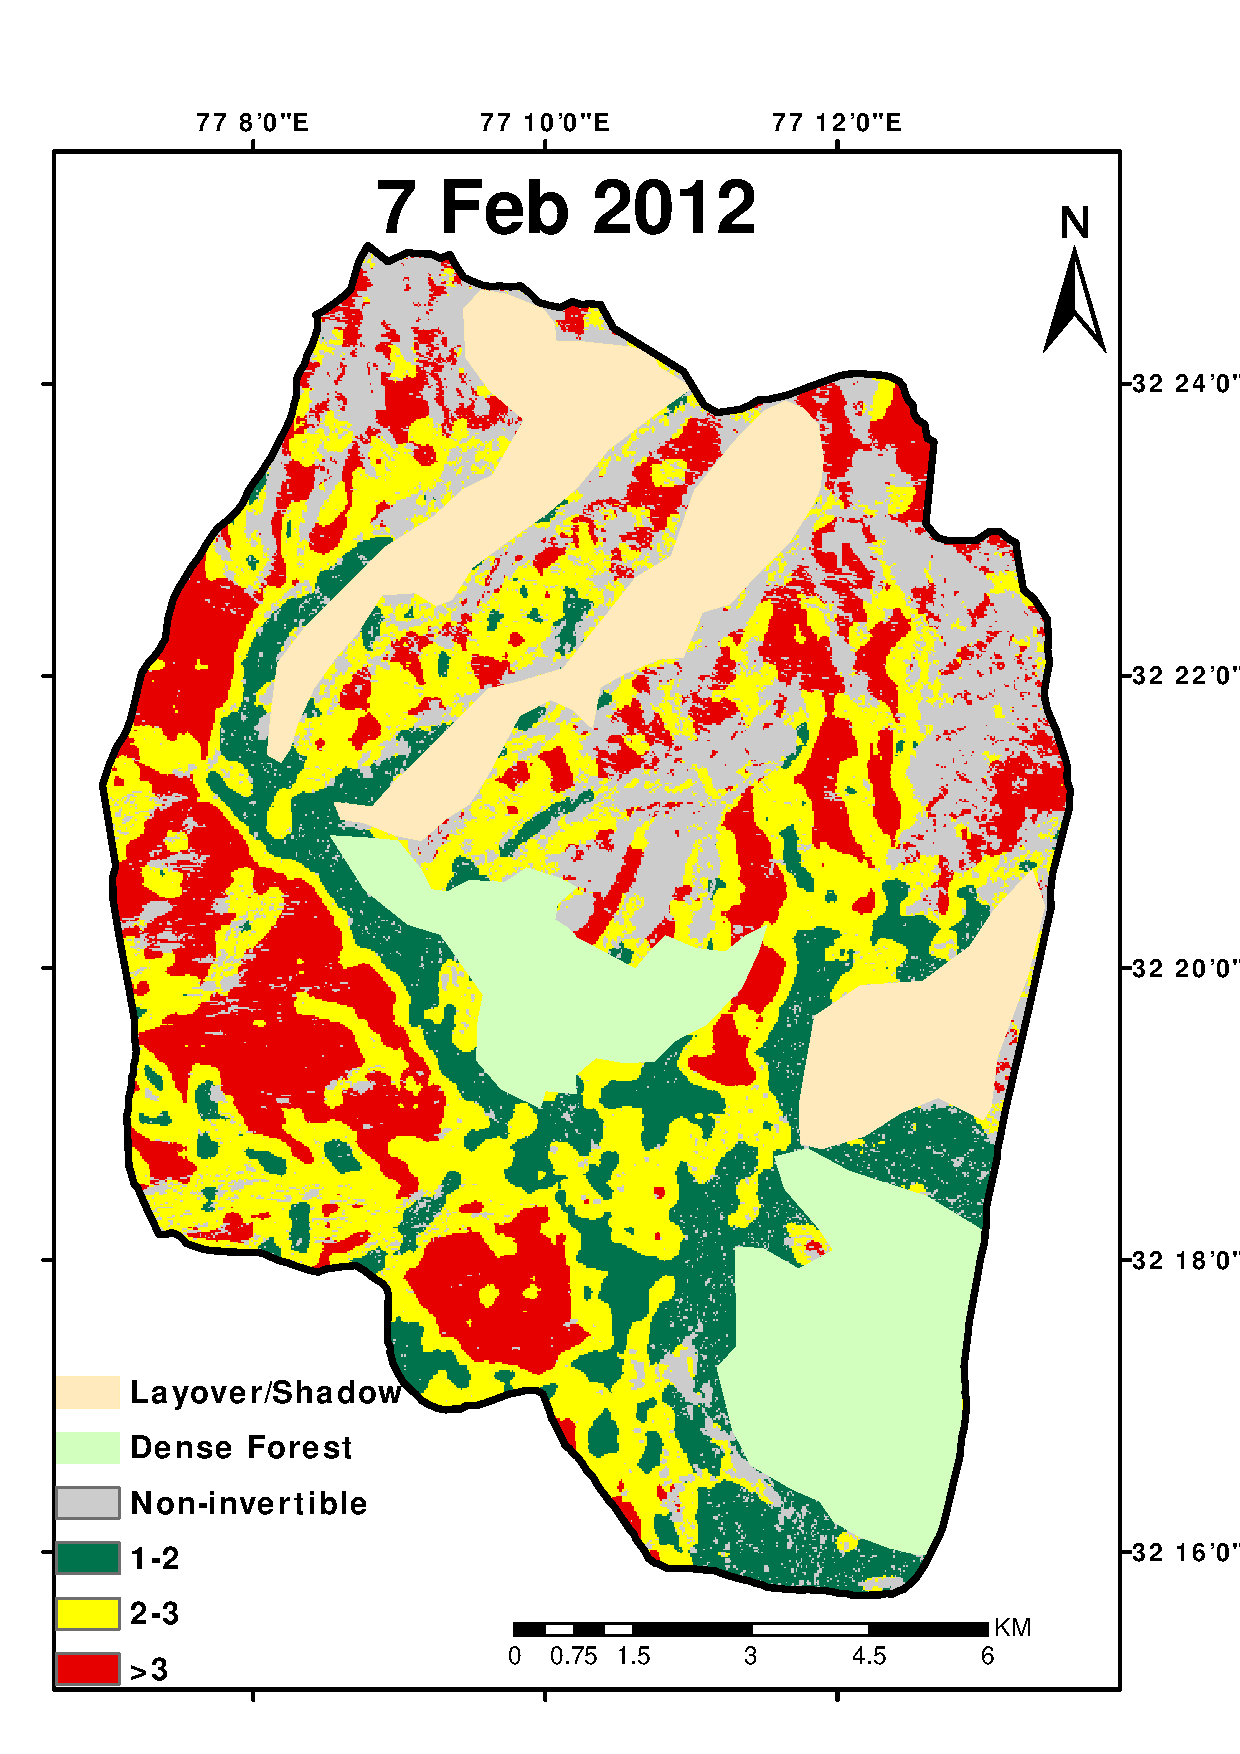
\includegraphics[width=0.49\textwidth]{Figures_sd/7Feb2012}}
%	\subfloat[]{\includegraphics[width=0.49\textwidth]{Figures_sd/8Feb2013}} \\
%	\subfloat[]{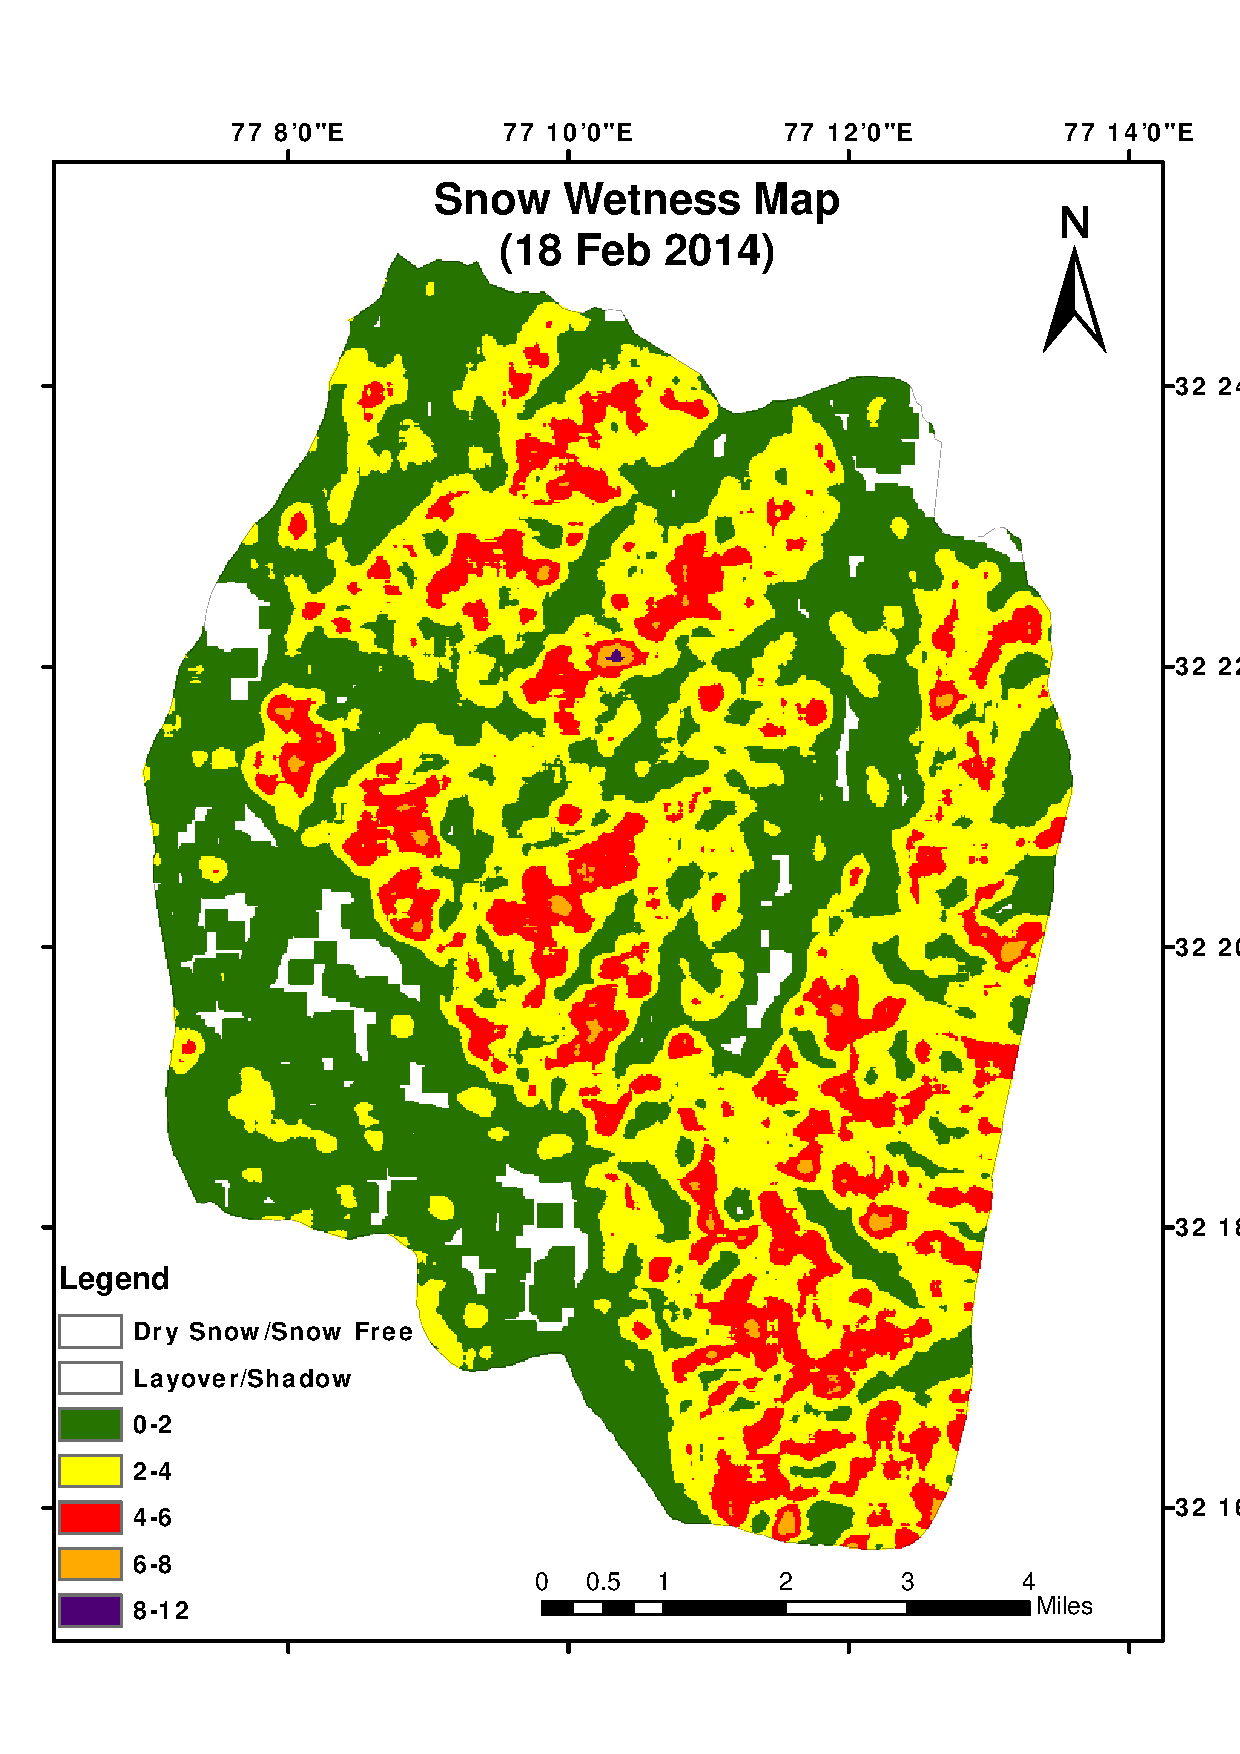
\includegraphics[width=0.49\textwidth]{Figures_sd/18Feb2014}}
%	\caption{Snow density maps derived from the proposed methodology. (For figure (c): RADARSAT-2 Data and Products ©MacDonald, Dettwiler and Associates Ltd. (2014) $-$ All Rights Reserved. RADARSAT is an official trademark of the Canadian Space Agency)}
%	\label{fig:proposed_results}
%\end{figure*}
%
%\begin{table}[!th]
%	\caption{Percentage of area with snow density range}
%	\begin{center}
%		\begin{tabular}{|c|c|c|c|} \hline
%			Snow Density Range (gcm$^{-3}$) & \multicolumn{3}{c|}{Area $\%$} \\
%			\cline{2-4}
%			& 7 Feb. 2012 & 8 Feb. 2013 & 18 Feb. 2014 \\ \hline
%			0.0--0.05 &	1.38 &	2.86 &	1.84 \\ \hline
%			0.05--0.1 &	0.73 &	4.15 &	0.98 \\ \hline
%			0.1--0.15 &	3.10 &	4.75 &	3.65 \\ \hline
%			0.15--0.2 &	5.79 &	5.70 &	5.07  \\ \hline
%			0.2--0.25 &	14.00 &	7.17 &	9.03 \\ \hline
%			0.25--0.3 &	20.28 &	7.20 &	14.24 \\ \hline
%			0.3--0.35 &	11.80 &	3.78 &	11.01 \\ \hline
%			0.35--0.4 &	4.02 &	0.92 &	5.10 \\ \hline
%			0.4--0.45 &	1.82 &	0.15 &	2.87 \\ \hline
%			0.45--0.5 &	0.37 &	0.01 &	1.13 \\ \hline
%			\hline		
%			Dense forest cover &	12.59 &	12.59 &	12.59 \\ \hline
%			Layover/Shadow &	12.67 &	12.67 &	15.42 \\ \hline
%			Snow free/Wet snow &	11.42 &	38.06 &	17.06 \\ \hline
%		\end{tabular}
%	\end{center}
%	\label{table:snow_density_range}
%\end{table}
%
%\begin{figure*}[!thbp]
%	\centering
%	\subfloat[]{\includegraphics[width=0.49\textwidth]{Figures_sd/Temp_variability_2012}} \hspace{0.1cm}
%	\subfloat[]{\includegraphics[width=0.49\textwidth]{Figures_sd/windspeed_variability_2012}} \\
%	\subfloat[]{\includegraphics[width=0.49\textwidth]{Figures_sd/Temp_variability_observatories_2013}}\hspace{0.1cm} 
%	\subfloat[]{\includegraphics[width=0.49\textwidth]{Figures_sd/Temp_variability_observatories_2014}} 	
%	\caption{(a) Temporal variation of temperatures over Dhundhi in Feb. 2012; (b) Temporal variation of wind speed over Dhundhi in Feb. 2012; (c)-(d) Temporal variation of minimum and maximum temperatures over all the three observatories in Feb 2013 and 2014 respectively}
%	\label{fig:multi_temp_plots}
%\end{figure*}
%
%\begin{figure*}[!thbp]
%	\centering
%	\subfloat[]{\includegraphics[width=0.49\textwidth]{Figures_sd/Temp_variability_jan_2015}}
%	\subfloat[]{\includegraphics[width=0.49\textwidth]{Figures_sd/Temp_variability_feb_2015}} \\
%	\subfloat[]{\includegraphics[width=0.49\textwidth]{Figures_sd/Temp_variability_mar_20151}} 
%	\caption{Temporal variation of average local temperature over the study area in (a) Jan 2015; (b) Feb 2015; (c) March 2015 (the data were taken from the site:http://www.accuweather.com as on 17 April 2015)}
%	\label{fig:temp_plots_2015}
%\end{figure*}
%During the same period in the following year (8 Feb. 2013), the density was estimated in the range of 0.2--0.3~gcm$^{-3}$ as shown in Fig.~\ref{fig:proposed_results}(b). This range of density values covers around 15$\%$ of the entire study area as shown in Table.~\ref{table:snow_density_range}. However, snow free/wet snow regions in the snow density map were around 38$\%$ as seen in Table.~\ref{table:snow_density_range}. This might be because of the maximum temperature recorded on 7 Feb. 2013. The observed temperatures at the Bahang, Solang and Dhundhi observatories on 7 Feb. 2013 were 11$^\circ$C, 7$^\circ$C and 6$^\circ$C (Fig.~\ref{fig:multi_temp_plots}(c)) respectively which were higher than 2012. However, It can be observed that the snow density values are lower than the previous year (7 Feb. 2012). This may be because of the fresh snow fall on 6 Feb. 2013. Even though high temperature was observed on 7 Feb. 2013, the snowpack might not have compacted firmly during the acquisition on 8 Feb. 2013 as compared to the multiple melt-freeze condition in 2012. 
%
%The estimated snow density map and the observatory measurements for the 18 Feb. 2014 data (Fig.~\ref{fig:proposed_results}(c)) shows a similar trend as that of 7 Feb. 2012. Unlike the 7 and 8 Feb, the 18 Feb. 2014 data was acquired in an ascending pass. It can be seen in Table.~\ref{table:snow_density_range} that 34$\%$ of the area was covered with the snow density values in the range of 0.2--0.35~gcm$^{-3}$. There was no fresh snow fall recorded for a week prior to the acquisition on 18 Feb. 2014. Moreover, a large variation can also be observed between the maximum and the minimum temperatures on 18 Feb. 2014 (Fig.~\ref{fig:multi_temp_plots}(d)). So the old snowpack has undergone multiple melt-refreeze process, which has increased the snowpack grain size and consequently the snow density. 
%
%The Radarsat-2 data acquired with the same geometry on 29 Jan, 22 Feb and 18 Mar. 2015 were used to analyze the snow density changes within a season. The snow density map of 29 Jan 2015 (Fig.~\ref{fig:multi_temp_density}(a)) indicates that the study area was completely covered with fresh snow. The estimated snow density values are less than 0.1 gcm$^{-3}$ in most of the areas as shown in Fig.~\ref{fig:multi_temp_density}(a). Generally, by the end of January, high amount of snow precipitation occurs in the Indian Himalaya. This is reflected in the map with low snow density values. The local averaged temperature plot (Fig.~\ref{fig:temp_plots_2015}(a)), shows that the temperature drops to 4$^\circ$C during the acquisition day. This is the lowest temperature recorded during that particular week which may be because of fresh snowfall on that day. 
%
%\begin{figure*}[!thbp]
%	\centering
%	\includegraphics[width=\textwidth]{Figures_sd/temporal_variability_SD}
%	\caption{Temporal variation of snow density in a season. (RADARSAT-2 Data and Products ©MacDonald, Dettwiler and Associates Ltd. (2014) $--$ All Rights Reserved. RADARSAT is an official trademark of the Canadian Space Agency)}
%	\label{fig:multi_temp_density}
%\end{figure*}
%
%The estimated snow density values were more than 0.2 gcm$^{-3}$ for most of the study area on 22 Feb. 2015 as shown in Fig.~\ref{fig:multi_temp_density}(b). Normally in February, snowfall occurs and large variations between the minimum and the maximum temperatures are observed within a day. Hence, considerable melting and refreezing occurs in the snowpack which increases the snow density. As observed in Fig.~\ref{fig:temp_plots_2015}(b), the averaged local temperature before the acquisition day was recorded at 12$^\circ$C. So, the snow surface melt might have refrozen during the descending pass acquisition (6.14 AM local IST). 
%
%Snow density map of 18 Mar. 2015 shows that $>$ 0.3 gcm$^{-3}$ of snow density values are observed in most of the study area as compared to the snow density map of February. Normally in March, the snowfall stops and the snowpack starts to melt. The white areas in this map possibly represents wet snow. This can be attributed to high temperature (Fig.~\ref{fig:temp_plots_2015}(c)) which may have melted the snow surface.
%
%\begin{figure*}[!thbp]
%	\centering
%	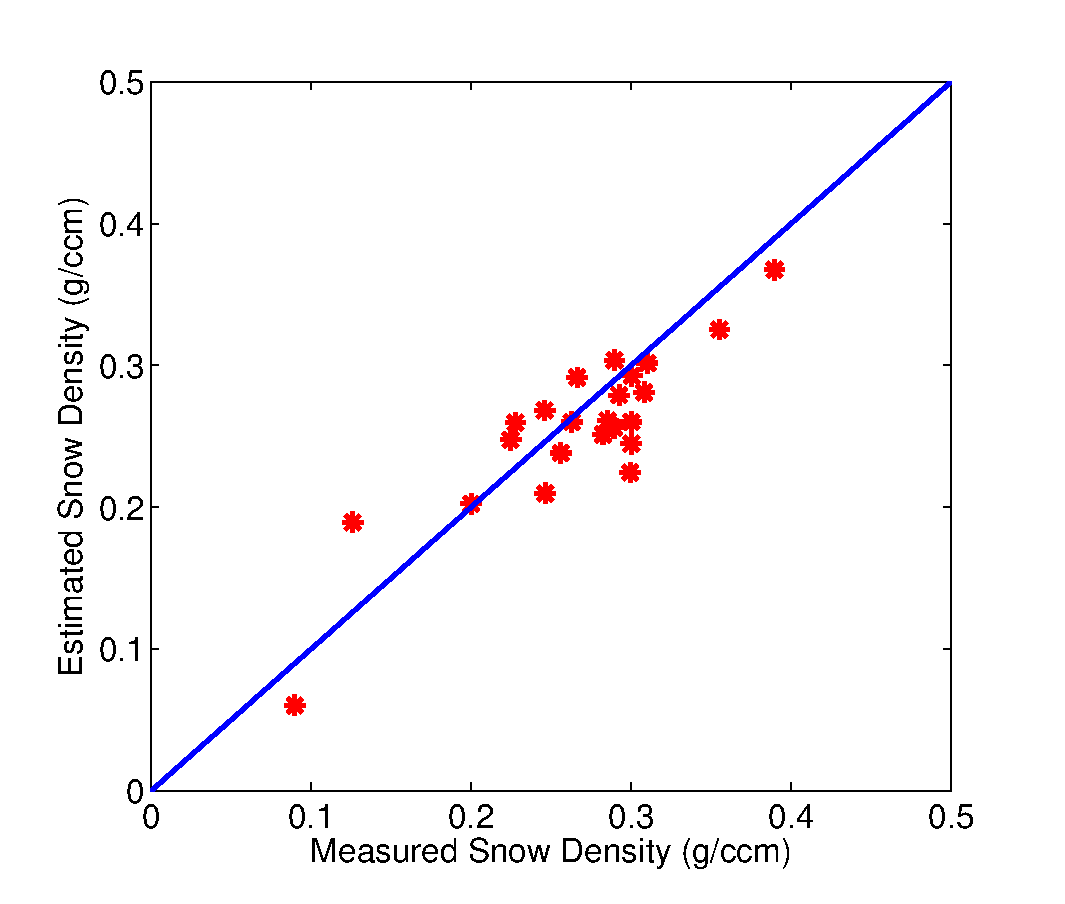
\includegraphics[width=0.5\textwidth]{Figures_sd/snow_density_validation}
%	\caption{Comparison of the snow densities estimated by the proposed methodology and in-situ measurements.}
%	\label{fig:validation_plot}
%\end{figure*} 
%
%A total of 23 near-real time in-situ measurements were collected with the satellite data for three consecutive years to validate the proposed snow density estimation algorithm. The snow densities estimated by the proposed methodology and measured in the field are plotted in Fig.~\ref{fig:validation_plot}. The mean absolute error (MAE) of  the proposed method is 0.027~gcm$^{-3}$ and the root mean square error (RMSE) is 0.032~gcm$^{-3}$. 
%
%\section{Conclusion}
%\label{S:5}
%
%In this work we have proposed a new methodology for snow density estimation from full-polarimetric SAR data. The generalized volume parameter is derived from the double unitary transformation of the coherency matrix. This parameter was directly used to estimate the snowpack density. The proposed methodology is applied to three Radarsat-2 fine resolution full-polarimetric datasets acquired over the Indian Himalayan region for three consecutive years. Extensive field campaigns were conducted to collect near-real time snow density measurements along with the satellite data which have been used for validation of the proposed methodology. The mean absolute error (MAE) and the root mean square error (RMSE) are 0.027~gcm$^{-3}$ and 0.032~gcm$^{-3}$ respectively. The temporal snow density variation analysis in a same season have been done  using the proposed method. The proposed methodology can be further improved for low frequency bands which will take into account the snow-ground along with the snowpack volume scattering information.

%% Authors are advised to submit their bibtex database files. They are
%% requested to list a bibtex style file in the manuscript if they do
%% not want to use model1-num-names.bst.

%% References without bibTeX database:

% \begin{thebibliography}{00}

%% \bibitem must have the following form:
%%   \bibitem{key}...
%%

% \bibitem{}

% \end{thebibliography}




